\documentclass{article}
\usepackage{graphicx}
\usepackage{booktabs}
\usepackage{threeparttable}
\usepackage{makecell}
\usepackage{amsmath}
\usepackage{amssymb}
\usepackage{pdflscape}
\usepackage{float}
\usepackage{geometry}
\usepackage{caption}
\usepackage[colorlinks=true, linkcolor=blue, citecolor=blue, urlcolor=blue]{hyperref}
\geometry{margin=1in}

\title{Campaign Visits and Local Newspaper Coverage:\\
Evidence from U.S.\ Presidential Elections}
\author{Sitong Li}
\date{August 2025}

\begin{document}

\maketitle

\begin{abstract}
This paper examines whether campaign visits by presidential and vice-presidential candidates
increase the local newspaper coverage they receive.
Using a county-day panel covering 22 states over a full election cycle, I estimate two-way
fixed effects (TWFE) models that absorb time-invariant county characteristics and nationwide
news shocks.
The baseline OLS-log specification finds that a same-day visit is associated with a
statistically significant 13\% increase in local coverage.
An event study confirms that this effect is concentrated on the visit day itself, with no
evidence of anticipatory coverage or post-visit persistence---consistent with a causal
interpretation.
A Poisson pseudo-maximum likelihood (PPML) model, which better handles the zero-heavy,
right-skewed count outcome, yields a small and statistically insignificant estimate,
underscoring sensitivity to functional-form assumptions.
Robustness checks show that headline coverage does not respond significantly to visits, and
that the coverage boost is concentrated among Democratic-ticket appearances.
\end{abstract}


%-----------------------------------------------------------------------
\section{Data Description and Descriptive Statistics}
\label{sec:data}
%-----------------------------------------------------------------------

Campaign visits are among the most resource-intensive tools in a presidential candidate's
toolkit, yet their downstream effects on local media attention remain an open empirical
question.
This paper asks: \emph{does a campaign visit by a presidential or vice-presidential
candidate causally increase the amount of local newspaper coverage that candidate
receives?}

To address this question, I construct a county-day panel dataset as follows.
First, I exclude all non-major-party candidates.
Second, I reshape the data into long format so that each observation corresponds to a
single county on a single calendar date.
I then construct three new variables at the county-day level:
\begin{itemize}
    \item \texttt{visit\_ticket} $= 1$ if either the presidential or vice-presidential
          candidate visited the county on that date.
    \item \texttt{counts\_ticket} $=$ \texttt{counts\_Pres} $+$ \texttt{counts\_VP}\;
          (total mentions in local newspapers).
    \item \texttt{hcounts\_ticket} $=$ \texttt{hcounts\_Pres} $+$ \texttt{hcounts\_VP}\;
          (headline mentions).
\end{itemize}
Both candidate-level and ticket-level datasets are retained.
The ticket-level dataset serves as the primary sample; the candidate-level dataset is used
for robustness and heterogeneity checks.
Table~\ref{tab:desc_stats} reports basic descriptive statistics.

\begin{table}[htbp]
\centering
\caption{Average counts and headline counts on visit vs.\ non-visit days}
\label{tab:desc_stats}
\begin{tabular}{lrr}
\toprule
 & \textbf{counts\_ticket} & \textbf{hcounts\_ticket} \\
\midrule
No Visit & 3.96 & 0.78 \\
Visit    & 7.58 & 1.93 \\
\bottomrule
\end{tabular}
\end{table}

The dataset covers 22 states (matching the task description), all counties within those
states, and 366 unique days.
Even at the descriptive level, average mentions---both total and headline---are
substantially higher on visit days than on non-visit days.
The share of county-days with any visit is approximately 0.13\%, indicating that visits
are rare events that nonetheless tend to coincide with elevated press attention.

Figures~\ref{fig:visit_mentions}--\ref{fig:event_study_pattern7} illustrate the main
patterns in the data.
Figure~\ref{fig:visit_mentions} confirms that visits are associated with higher average
media mentions.
Figure~\ref{fig:whitehouse_effect} suggests that the party occupying the White House also
influences coverage intensity.
Figures~\ref{fig:event_study_pattern1}, \ref{fig:event_study_pattern3},
\ref{fig:event_study_pattern5}, and~\ref{fig:event_study_pattern7} show that mentions tend
to spike around visit dates, motivating the event study framework developed in
Section~\ref{sec:main}.

\begin{figure}[htbp]
    \centering
    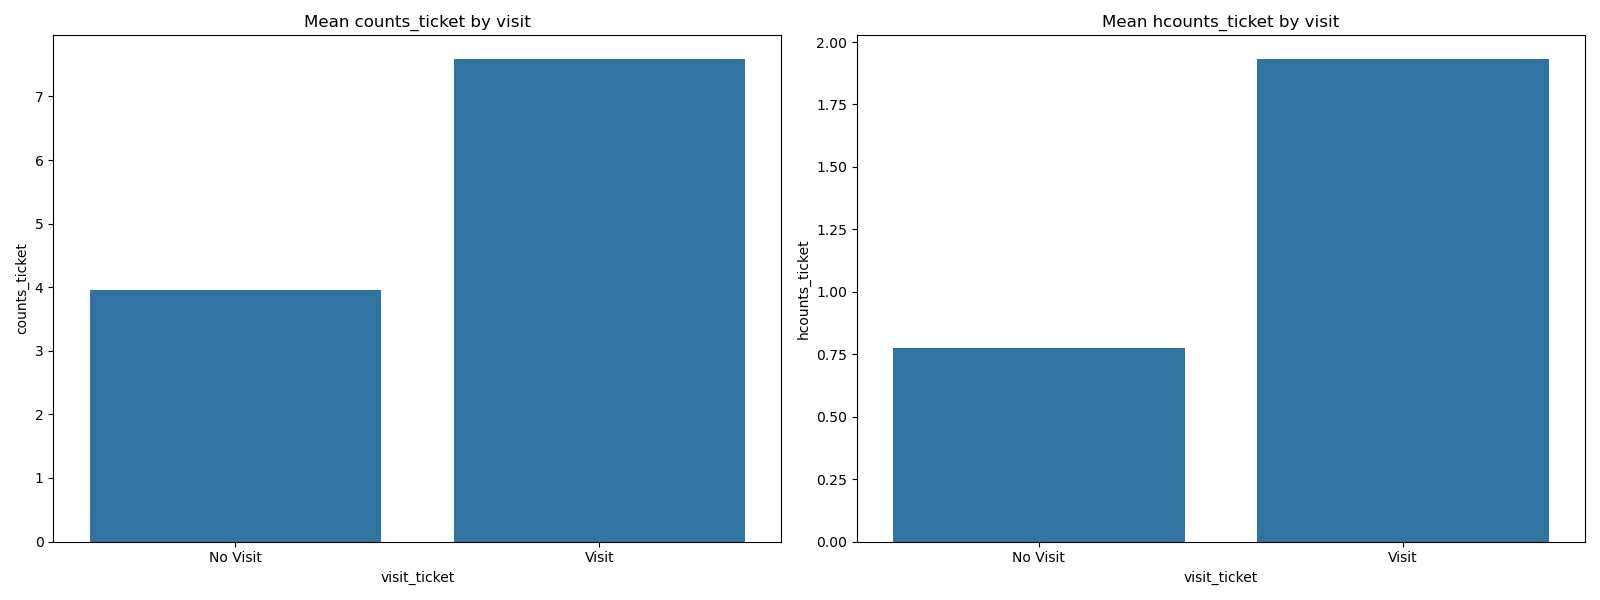
\includegraphics[width=0.8\textwidth]{plot/bar_mean.png}
    \caption{Average media mentions by visit status.}
    \label{fig:visit_mentions}
\end{figure}

\begin{figure}[htbp]
    \centering
    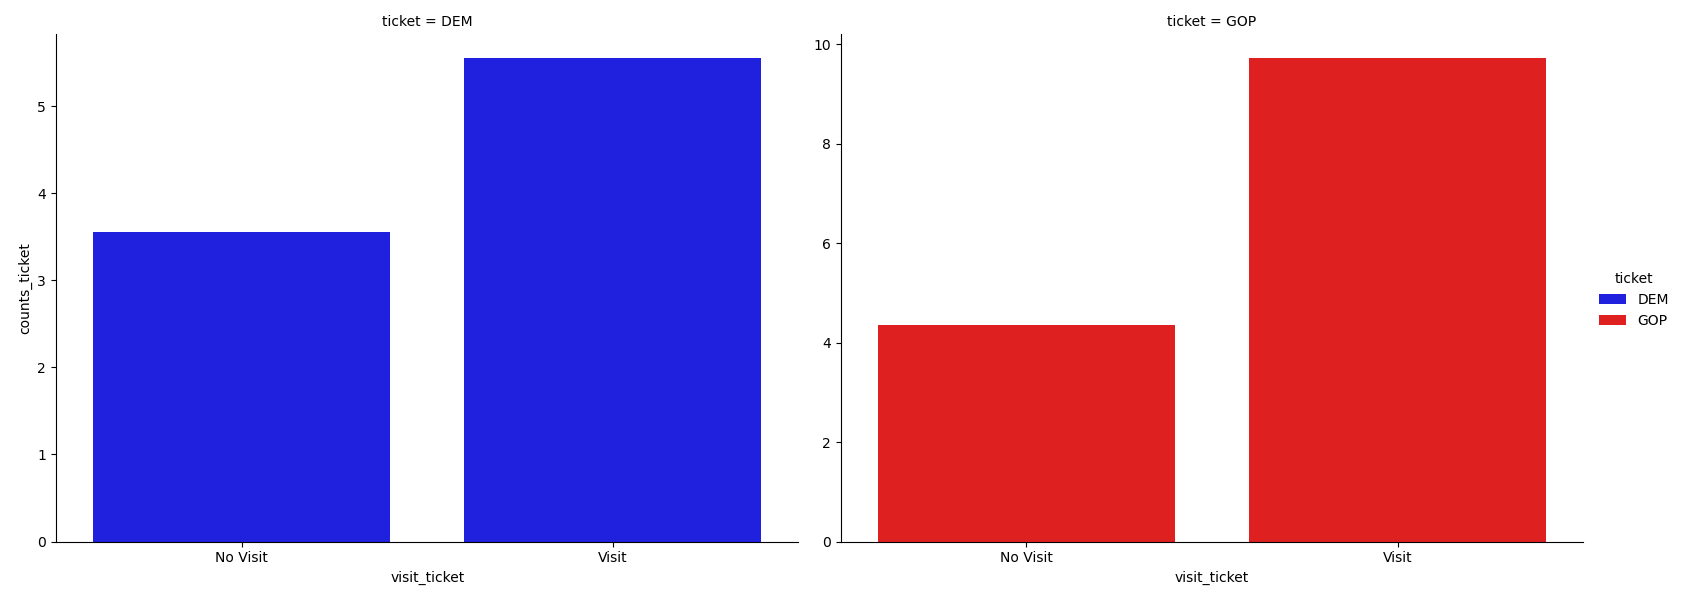
\includegraphics[width=0.8\textwidth]{plot/bar_party.png}
    \caption{Coverage intensity by party occupancy of the White House.}
    \label{fig:whitehouse_effect}
\end{figure}

\begin{figure}[htbp]
    \centering
    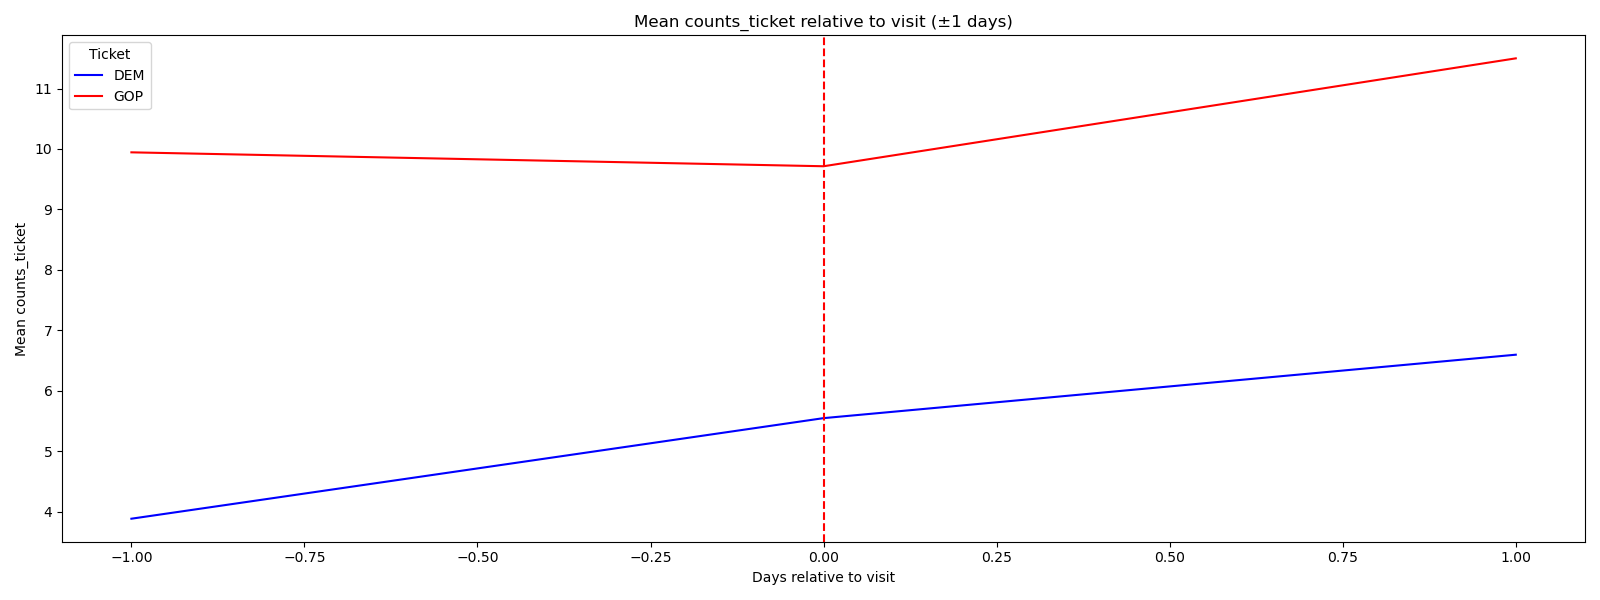
\includegraphics[width=0.8\textwidth]{plot/window_1.png}
    \caption{Media mentions around visit dates: $\pm1$-day window.}
    \label{fig:event_study_pattern1}
\end{figure}

\begin{figure}[htbp]
    \centering
    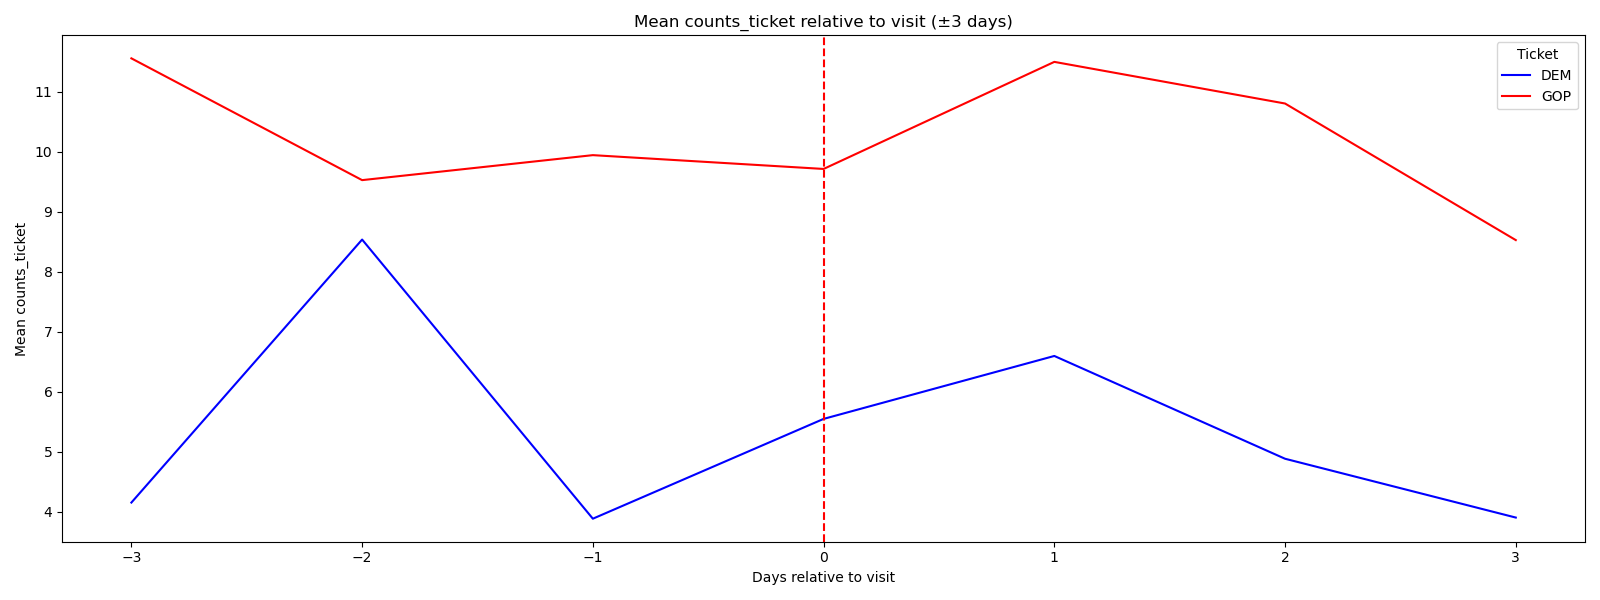
\includegraphics[width=0.8\textwidth]{plot/window_3.png}
    \caption{Media mentions around visit dates: $\pm3$-day window.}
    \label{fig:event_study_pattern3}
\end{figure}

\begin{figure}[htbp]
    \centering
    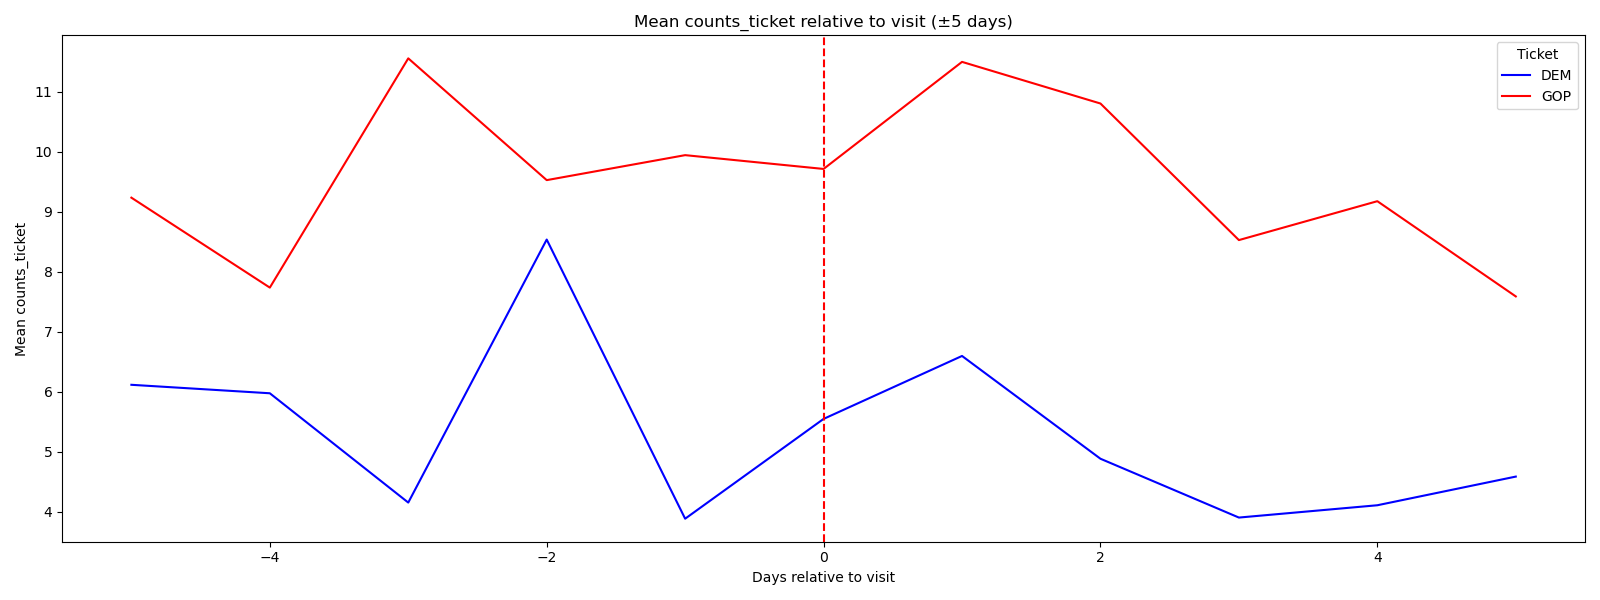
\includegraphics[width=0.8\textwidth]{plot/window_5.png}
    \caption{Media mentions around visit dates: $\pm5$-day window.}
    \label{fig:event_study_pattern5}
\end{figure}

\begin{figure}[htbp]
    \centering
    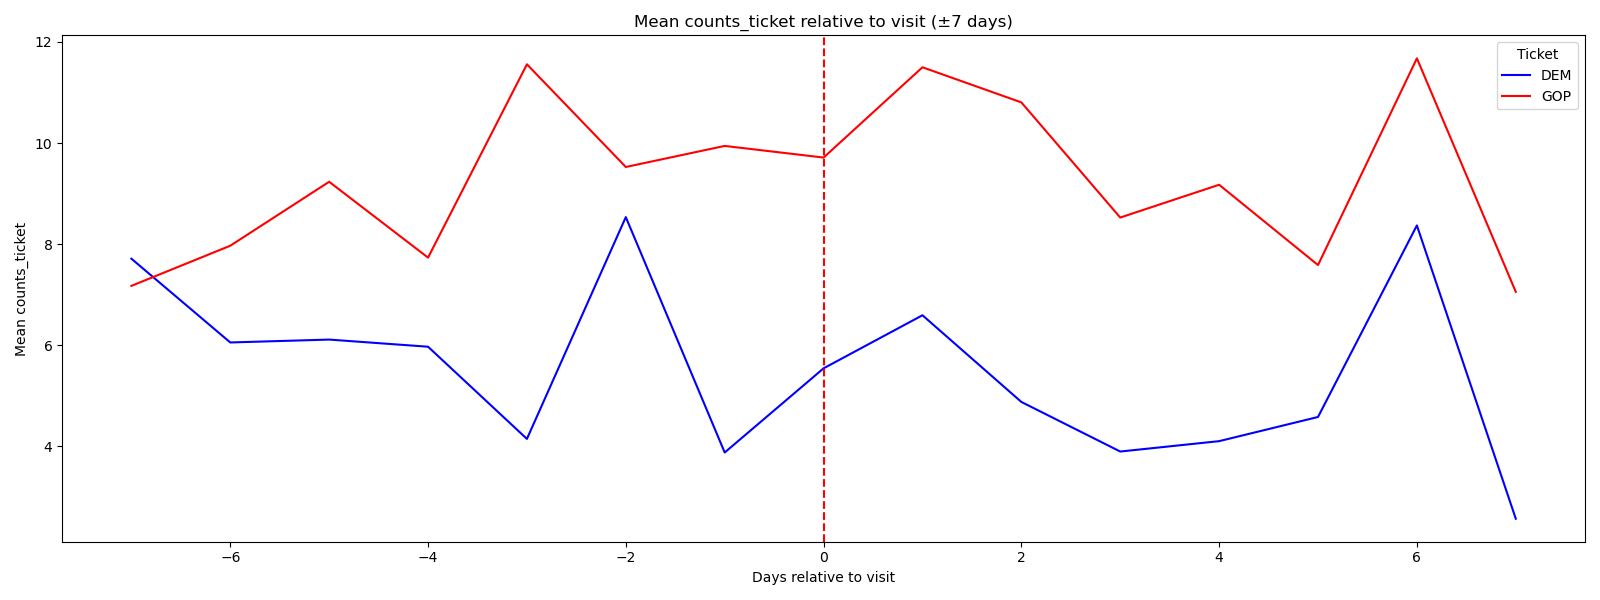
\includegraphics[width=0.8\textwidth]{plot/window_7.png}
    \caption{Media mentions around visit dates: $\pm7$-day window.}
    \label{fig:event_study_pattern7}
\end{figure}


%-----------------------------------------------------------------------
\section{Main Results}
\label{sec:main}
%-----------------------------------------------------------------------

\subsection*{Baseline Specification: Two-Way Fixed Effects}

To estimate the effect of campaign visits on newspaper coverage, I estimate the following
TWFE model at the ticket level:
\begin{equation}
\log\!\big(1+\text{Coverage}_{c,t}^{\text{ticket}}\big)
= \alpha_c + \theta_t + \beta \cdot \text{Visit}_{c,t}^{\text{ticket}} + \varepsilon_{c,t},
\label{eq:baseline}
\end{equation}
where $\alpha_c$ are \textbf{county fixed effects} that absorb persistent, time-invariant
differences in media intensity across counties, and $\theta_t$ are \textbf{date fixed
effects} that absorb nationwide news shocks and day-of-week patterns.
The dependent variable is $\log(1+\text{Coverage})$, so $\beta$ is a \textbf{semi-elasticity}:
the approximate percentage change in coverage associated with a visit.
Standard errors are clustered one-way at the county level (Column~1) or two-way at the
county and date levels (Column~2) to allow for correlated errors within each dimension.

\begin{table}[htbp]
\centering
\caption{Baseline estimates: effect of campaign visits on local newspaper coverage}
\label{tab:baseline}
\renewcommand\cellalign{t}
\begin{threeparttable}
\begin{tabular}{lcc}
\toprule
 & \multicolumn{2}{c}{$\log(1+\text{counts})$} \\
\cmidrule(lr){2-3}
 & (1) & (2) \\
\midrule
\addlinespace
Visit (Ticket) & \makecell{0.131* \\ (0.052)} & \makecell{0.131* \\ (0.051)} \\
\midrule
\addlinespace
Date FE        & $\checkmark$ & $\checkmark$ \\
County FE      & $\checkmark$ & $\checkmark$ \\
\midrule
\addlinespace
Observations   & 66,612 & 66,612 \\
S.E. clustered by & County & County $+$ Date \\
$R^2$          & 0.705 & 0.705 \\
$R^2$ Within   & 0.000 & 0.000 \\
\bottomrule
\end{tabular}
\begin{tablenotes}
\footnotesize
\item \textit{Notes}: $*$ $p<0.05$, $**$ $p<0.01$, $***$ $p<0.001$.
      Standard errors in parentheses.
\end{tablenotes}
\end{threeparttable}
\end{table}

The estimated coefficient on Visit (Table~\ref{tab:baseline}) implies that a campaign
visit is associated with roughly a \textbf{13\% increase} in same-day local newspaper
coverage for the ticket, relative to non-visit days, holding fixed county-level media
intensity and nationwide news shocks.
The effect is statistically significant at the 5\% level under both one-way and two-way
clustered standard errors.
The within-$R^2$ is small, reflecting that visits explain only a modest fraction of
within-county daily variation in coverage---expected given the many other factors that
drive news content.
Nonetheless, the positive and significant coefficient indicates that visits generate a
measurable boost in local press attention.


\subsection*{Count Model: Poisson Pseudo-Maximum Likelihood}

To complement the OLS-log specification, I estimate a Poisson pseudo-maximum likelihood
(PPML) model:
\begin{equation}
\mathbb{E}\big[\text{Coverage}_{c,t}^{\text{ticket}} \mid \cdot\big]
= \exp\!\big\{\alpha_c + \theta_t + \beta \cdot \text{Visit}_{c,t}^{\text{ticket}}\big\},
\label{eq:ppml}
\end{equation}
with county and date fixed effects and standard errors clustered at the county level.
PPML offers two advantages over the log-linear OLS model.
First, it handles zero-coverage days without the $\log(1+y)$ transformation, which can
introduce bias when the outcome has a large mass at zero.
Second, PPML yields consistent estimates under heteroskedasticity, making it well-suited
for right-skewed count outcomes such as media mentions.
Both properties are particularly relevant here, given that visit days are rare and the
outcome distribution is highly skewed.

\begin{table}[htbp]
\centering
\caption{PPML estimates: effect of campaign visits on local newspaper coverage}
\label{tab:ppml}
\renewcommand\cellalign{t}
\begin{threeparttable}
\begin{tabular}{lc}
\toprule
 & \multicolumn{1}{c}{Counts (Ticket, PPML)} \\
\cmidrule(lr){2-2}
 & (1) \\
\midrule
\addlinespace
Visit (Ticket) & \makecell{$-$0.039 \\ (0.064)} \\
\midrule
\addlinespace
Date FE        & $\checkmark$ \\
County FE      & $\checkmark$ \\
\midrule
\addlinespace
Observations     & 66,612 \\
S.E. clustered by & County \\
Log-Likelihood   & $-$124,860 \\
Pseudo $R^2$     & 0.999 \\
\bottomrule
\end{tabular}
\begin{tablenotes}
\footnotesize
\item \textit{Notes}: $*$ $p<0.05$, $**$ $p<0.01$, $***$ $p<0.001$.
      Standard errors in parentheses.
      Poisson family with log link; county and date fixed effects.
\end{tablenotes}
\end{threeparttable}
\end{table}

In contrast to the OLS-log result, the PPML estimate for Visit (Table~\ref{tab:ppml}) is
small, negative ($-0.039$), and statistically insignificant.
After controlling for county and date effects, we cannot reject the null hypothesis of no
visit effect under the count model specification.
The divergence between the two estimates likely reflects differences in how each model
handles zeros, distributional skewness, and influential observations.
Given the sparse and skewed nature of the outcome, the PPML result should be treated as a
conservative benchmark that tempers the OLS-log finding.


\subsection*{Event Study: Dynamic Effects of Campaign Visits}

To examine the \textbf{timing and persistence} of visit effects, I estimate an event study
specification:
\begin{equation}
\log\!\big(1+\text{Coverage}_{c,t}\big)
= \alpha_c + \theta_t + \sum_{\tau \neq -1} \beta_\tau \, D_{\tau,c,t} + \varepsilon_{c,t},
\label{eq:eventstudy}
\end{equation}
where $D_{\tau,c,t}$ is an indicator for being $\tau$ days relative to a visit, with
$\tau = -1$ (the day before the visit) omitted as the baseline.
Leads ($\tau < 0$) test for pre-existing trends; lags ($\tau > 0$) capture post-visit
persistence.
The event window is reset at each visit to avoid overlap across multiple visit events.

\begin{table}[htbp]
\centering
\caption{Event study estimates: dynamic effects of campaign visits on local newspaper
coverage}
\label{tab:eventstudy}
\renewcommand\cellalign{t}
\begin{threeparttable}
\begin{tabular}{lc}
\toprule
 & $\log(1+\text{counts})$ \\
 & (1) \\
\midrule
\addlinespace
$D_{-7}$ & \makecell{0.005 \\ (0.107)} \\
$D_{-6}$ & \makecell{0.097 \\ (0.107)} \\
$D_{-5}$ & \makecell{0.056 \\ (0.106)} \\
$D_{-4}$ & \makecell{$-$0.006 \\ (0.105)} \\
$D_{-3}$ & \makecell{0.084 \\ (0.109)} \\
$D_{-2}$ & \makecell{0.162 \\ (0.103)} \\
$D_{0}$  & \makecell{0.205* \\ (0.094)} \\
$D_{1}$  & \makecell{0.064 \\ (0.117)} \\
$D_{2}$  & \makecell{0.099 \\ (0.102)} \\
$D_{3}$  & \makecell{0.063 \\ (0.106)} \\
$D_{4}$  & \makecell{$-$0.022 \\ (0.104)} \\
$D_{5}$  & \makecell{0.039 \\ (0.108)} \\
$D_{6}$  & \makecell{0.071 \\ (0.111)} \\
$D_{7}$  & \makecell{$-$0.113 \\ (0.101)} \\
\midrule
\addlinespace
Date FE        & $\checkmark$ \\
County FE      & $\checkmark$ \\
\midrule
\addlinespace
Observations   & 1,105 \\
S.E. type      & Heteroskedasticity-robust \\
$R^2$          & 0.817 \\
$R^2$ Within   & 0.018 \\
\bottomrule
\end{tabular}
\begin{tablenotes}
\footnotesize
\item \textit{Notes}: $*$ $p<0.05$, $**$ $p<0.01$, $***$ $p<0.001$.
      Standard errors in parentheses.
      The omitted category is $\tau = -1$ (the day before the visit).
\end{tablenotes}
\end{threeparttable}
\end{table}

\begin{figure}[htbp]
    \centering
    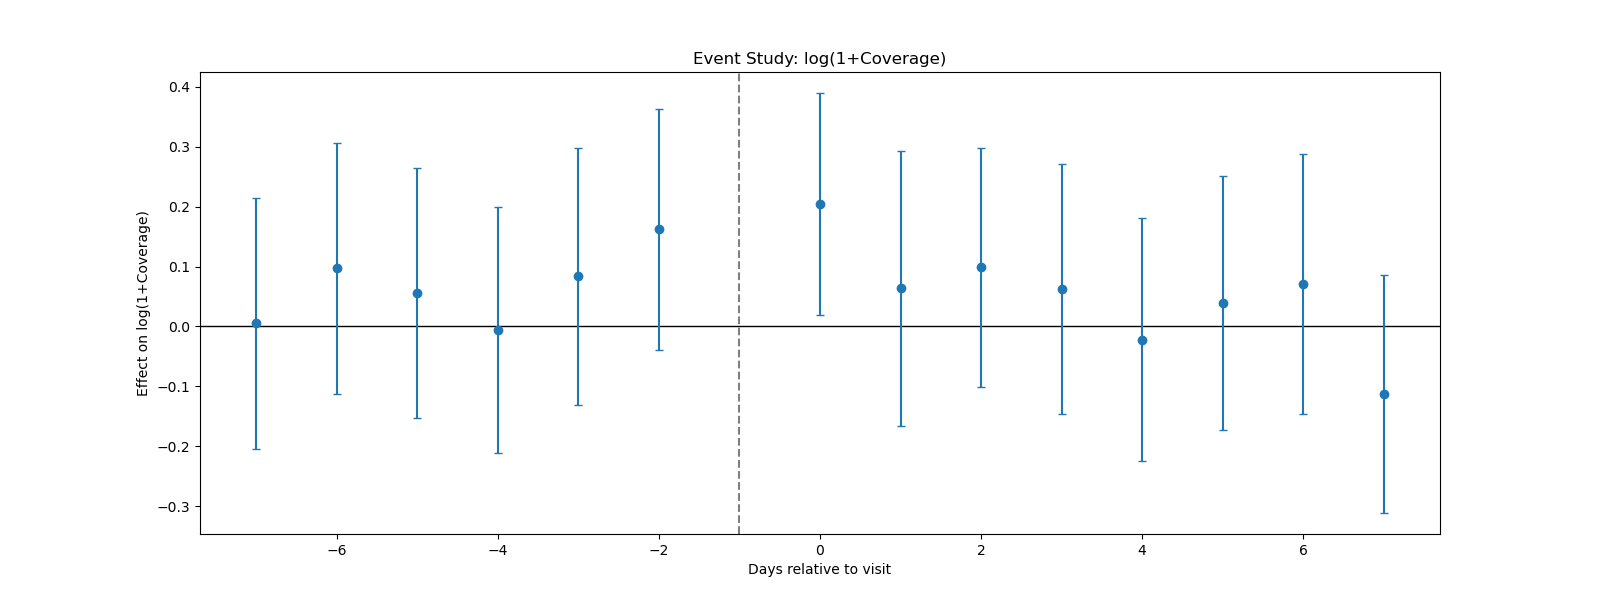
\includegraphics[width=0.85\textwidth]{plot/res_plot.png}
    \caption{Event study: dynamic effects of campaign visits on local newspaper coverage.
    The dashed vertical line marks the visit day ($\tau = 0$).
    Coefficients are from Equation~\eqref{eq:eventstudy}; bands show 95\% confidence
    intervals.}
    \label{fig:eventstudyplot}
\end{figure}

The event study results, reported in Table~\ref{tab:eventstudy} and
Figure~\ref{fig:eventstudyplot}, support a causal interpretation of the baseline result.
All pre-visit coefficients ($\tau \leq -2$) are small and statistically indistinguishable
from zero, providing no evidence of pre-existing trends or anticipatory coverage in the
week leading up to the visit---a key requirement for causal identification.
On the visit day itself ($\tau = 0$), coverage rises by approximately 20\% relative to the
omitted baseline, significant at the 5\% level.
Post-visit coefficients are individually insignificant and fluctuate around zero, indicating
that the media boost is short-lived and does not persist beyond the visit day.

Overall, the event study confirms that campaign visits generate a sharp, concentrated spike
in local newspaper coverage, with no meaningful anticipatory or carry-over effects.


%-----------------------------------------------------------------------
\section{Robustness Checks}
\label{sec:robust}
%-----------------------------------------------------------------------

To assess the robustness of the main results, I conduct two additional tests.

\paragraph{Headline Coverage.}
Table~\ref{tab:headline} replaces total mentions with headline coverage as the dependent
variable.
The coefficient on Visit (Ticket) is positive but small and statistically insignificant,
suggesting that visits do not robustly drive high-visibility headline placement.
This may reflect the rarity of headline coverage---which reduces statistical power---or
that campaign visits tend to generate routine news items rather than front-page stories.
The latter interpretation would qualify the main finding: while visits boost total mentions,
the additional coverage may be of limited salience.

\begin{table}[H]
\centering
\caption{Headline coverage as dependent variable}
\label{tab:headline}
\renewcommand\cellalign{t}
\begin{threeparttable}
\begin{tabular}{lc}
\toprule
 & $\log(1+\text{headline counts})$ \\
 & (1) \\
\midrule
\addlinespace
Visit (Ticket) & \makecell{0.059 \\ (0.057)} \\
\midrule
\addlinespace
Date FE        & $\checkmark$ \\
County FE      & $\checkmark$ \\
\midrule
\addlinespace
Observations   & 66,612 \\
S.E. type      & Heteroskedasticity-robust \\
$R^2$          & 0.482 \\
$R^2$ Within   & 0.000 \\
\bottomrule
\end{tabular}
\begin{tablenotes}
\footnotesize
\item \textit{Notes}: $*$ $p<0.05$, $**$ $p<0.01$, $***$ $p<0.001$.
      Standard errors in parentheses.
\end{tablenotes}
\end{threeparttable}
\end{table}

\paragraph{Opponent and Spillover Effects.}
I next estimate models that include both own-ticket and opponent-ticket visit indicators,
estimated separately for each party.
Results are reported in Tables~\ref{tab:opp_gop} and~\ref{tab:opp_dem}.

For \textit{GOP coverage} (Table~\ref{tab:opp_gop}): a GOP ticket visit is associated with
a 6.3\% increase in local GOP coverage, and a Democratic ticket visit with a 9.3\%
increase---neither effect is statistically significant at conventional levels.

For \textit{Democratic coverage} (Table~\ref{tab:opp_dem}): a Democratic ticket visit is
associated with a 22.5\% increase in local coverage, significant at the 1\% level.
In contrast, a GOP ticket visit is associated with a 10.1\% decrease in Democratic
coverage, though this effect is not statistically significant.

These results reveal an asymmetry: Democratic candidates receive a strong and statistically
significant coverage boost from same-day visits, while the corresponding effect for GOP
candidates is smaller and imprecisely estimated.
Neither party experiences a robust spillover from the opponent's visit.

\begin{table}[H]
\centering
\caption{Opponent and spillover effects: GOP coverage model}
\label{tab:opp_gop}
\renewcommand\cellalign{t}
\begin{threeparttable}
\begin{tabular}{lc}
\toprule
 & \multicolumn{1}{c}{$\log(1+\text{Counts}_{\text{GOP}})$} \\
\cmidrule(lr){2-2}
 & (1) \\
\midrule
\addlinespace
Visit (GOP Ticket) & \makecell{0.063 \\ (0.069)} \\
Visit (DEM Ticket) & \makecell{0.093 \\ (0.089)} \\
\midrule
\addlinespace
Date FE   & $\checkmark$ \\
County FE & $\checkmark$ \\
\midrule
\addlinespace
Observations & 33,306 \\
S.E. type    & Heteroskedasticity-robust \\
$R^2$        & 0.732 \\
$R^2$ Within & 0.000 \\
\bottomrule
\end{tabular}
\begin{tablenotes}
\footnotesize
\item \textit{Notes}: $*$ $p<0.05$, $**$ $p<0.01$, $***$ $p<0.001$.
      Standard errors in parentheses.
\end{tablenotes}
\end{threeparttable}

\end{table}

\begin{table}[H]
\centering
\caption{Opponent and spillover effects: DEM coverage model}
\label{tab:opp_dem}
\renewcommand\cellalign{t}
\begin{threeparttable}
\begin{tabular}{lcc}
\toprule
 & log_counts \\
 & (1) \\
\midrule
\addlinespace
visit_ticket & \makecell{0.225*** \\ (0.066)} \\
opp_visit & \makecell{-0.101 \\ (0.098)} \\
\midrule
\addlinespace
date_str & x \\
countycode & x \\
\midrule
\addlinespace
Observations & 33306 \\
S.E. type & hetero \\
$R^2$ & 0.721 \\
$R^2$ Within & 0.000 \\
\bottomrule
\end{tabular}
\footnotesize Significance levels: $*$ p $<$ 0.05, $**$ p $<$ 0.01, $***$ p $<$ 0.001. Format of coefficient cell: Coefficient 
 (Std. Error)
\end{threeparttable}
\end{table}


%-----------------------------------------------------------------------
\section{Conclusion}
%-----------------------------------------------------------------------

This paper finds that campaign visits by presidential or vice-presidential candidates
generate a measurable, but modest, short-lived, and model-dependent increase in local
newspaper coverage.
Under a baseline TWFE model, a visit is associated with a statistically significant 13\%
increase in same-day coverage.
An event study confirms that this effect is concentrated on the visit day, with no evidence
of anticipatory coverage in the preceding week or persistence in the days that follow.
However, a Poisson count model---which better accounts for the zero-heavy, skewed nature of
the outcome---yields a small and insignificant estimate, highlighting the sensitivity of
the finding to functional-form assumptions.

Robustness checks further qualify the main result.
Headline coverage does not respond significantly to visits, suggesting that the boost in
total mentions reflects incremental rather than prominent press attention.
Moreover, the significant own-visit effect is concentrated among Democratic-ticket
appearances, with no analogous effect detected for Republican candidates.

Taken together, the evidence supports the conclusion that campaign visits generate a brief
spike in local press coverage, but this effect is fragile across estimators, concentrated
on the visit day, and asymmetric across parties.

\end{document}
